\subsection{Verspleißen von Faserenden}
Nach dem Entfernen der Schutzschicht mit einer speziellen Zange wurde das Faserende mit einem Reinigungstuch und Alkohol von den letzten Rückständen des Coatings befreit.\\

% \begin{figure}[H]
%   \centering
%   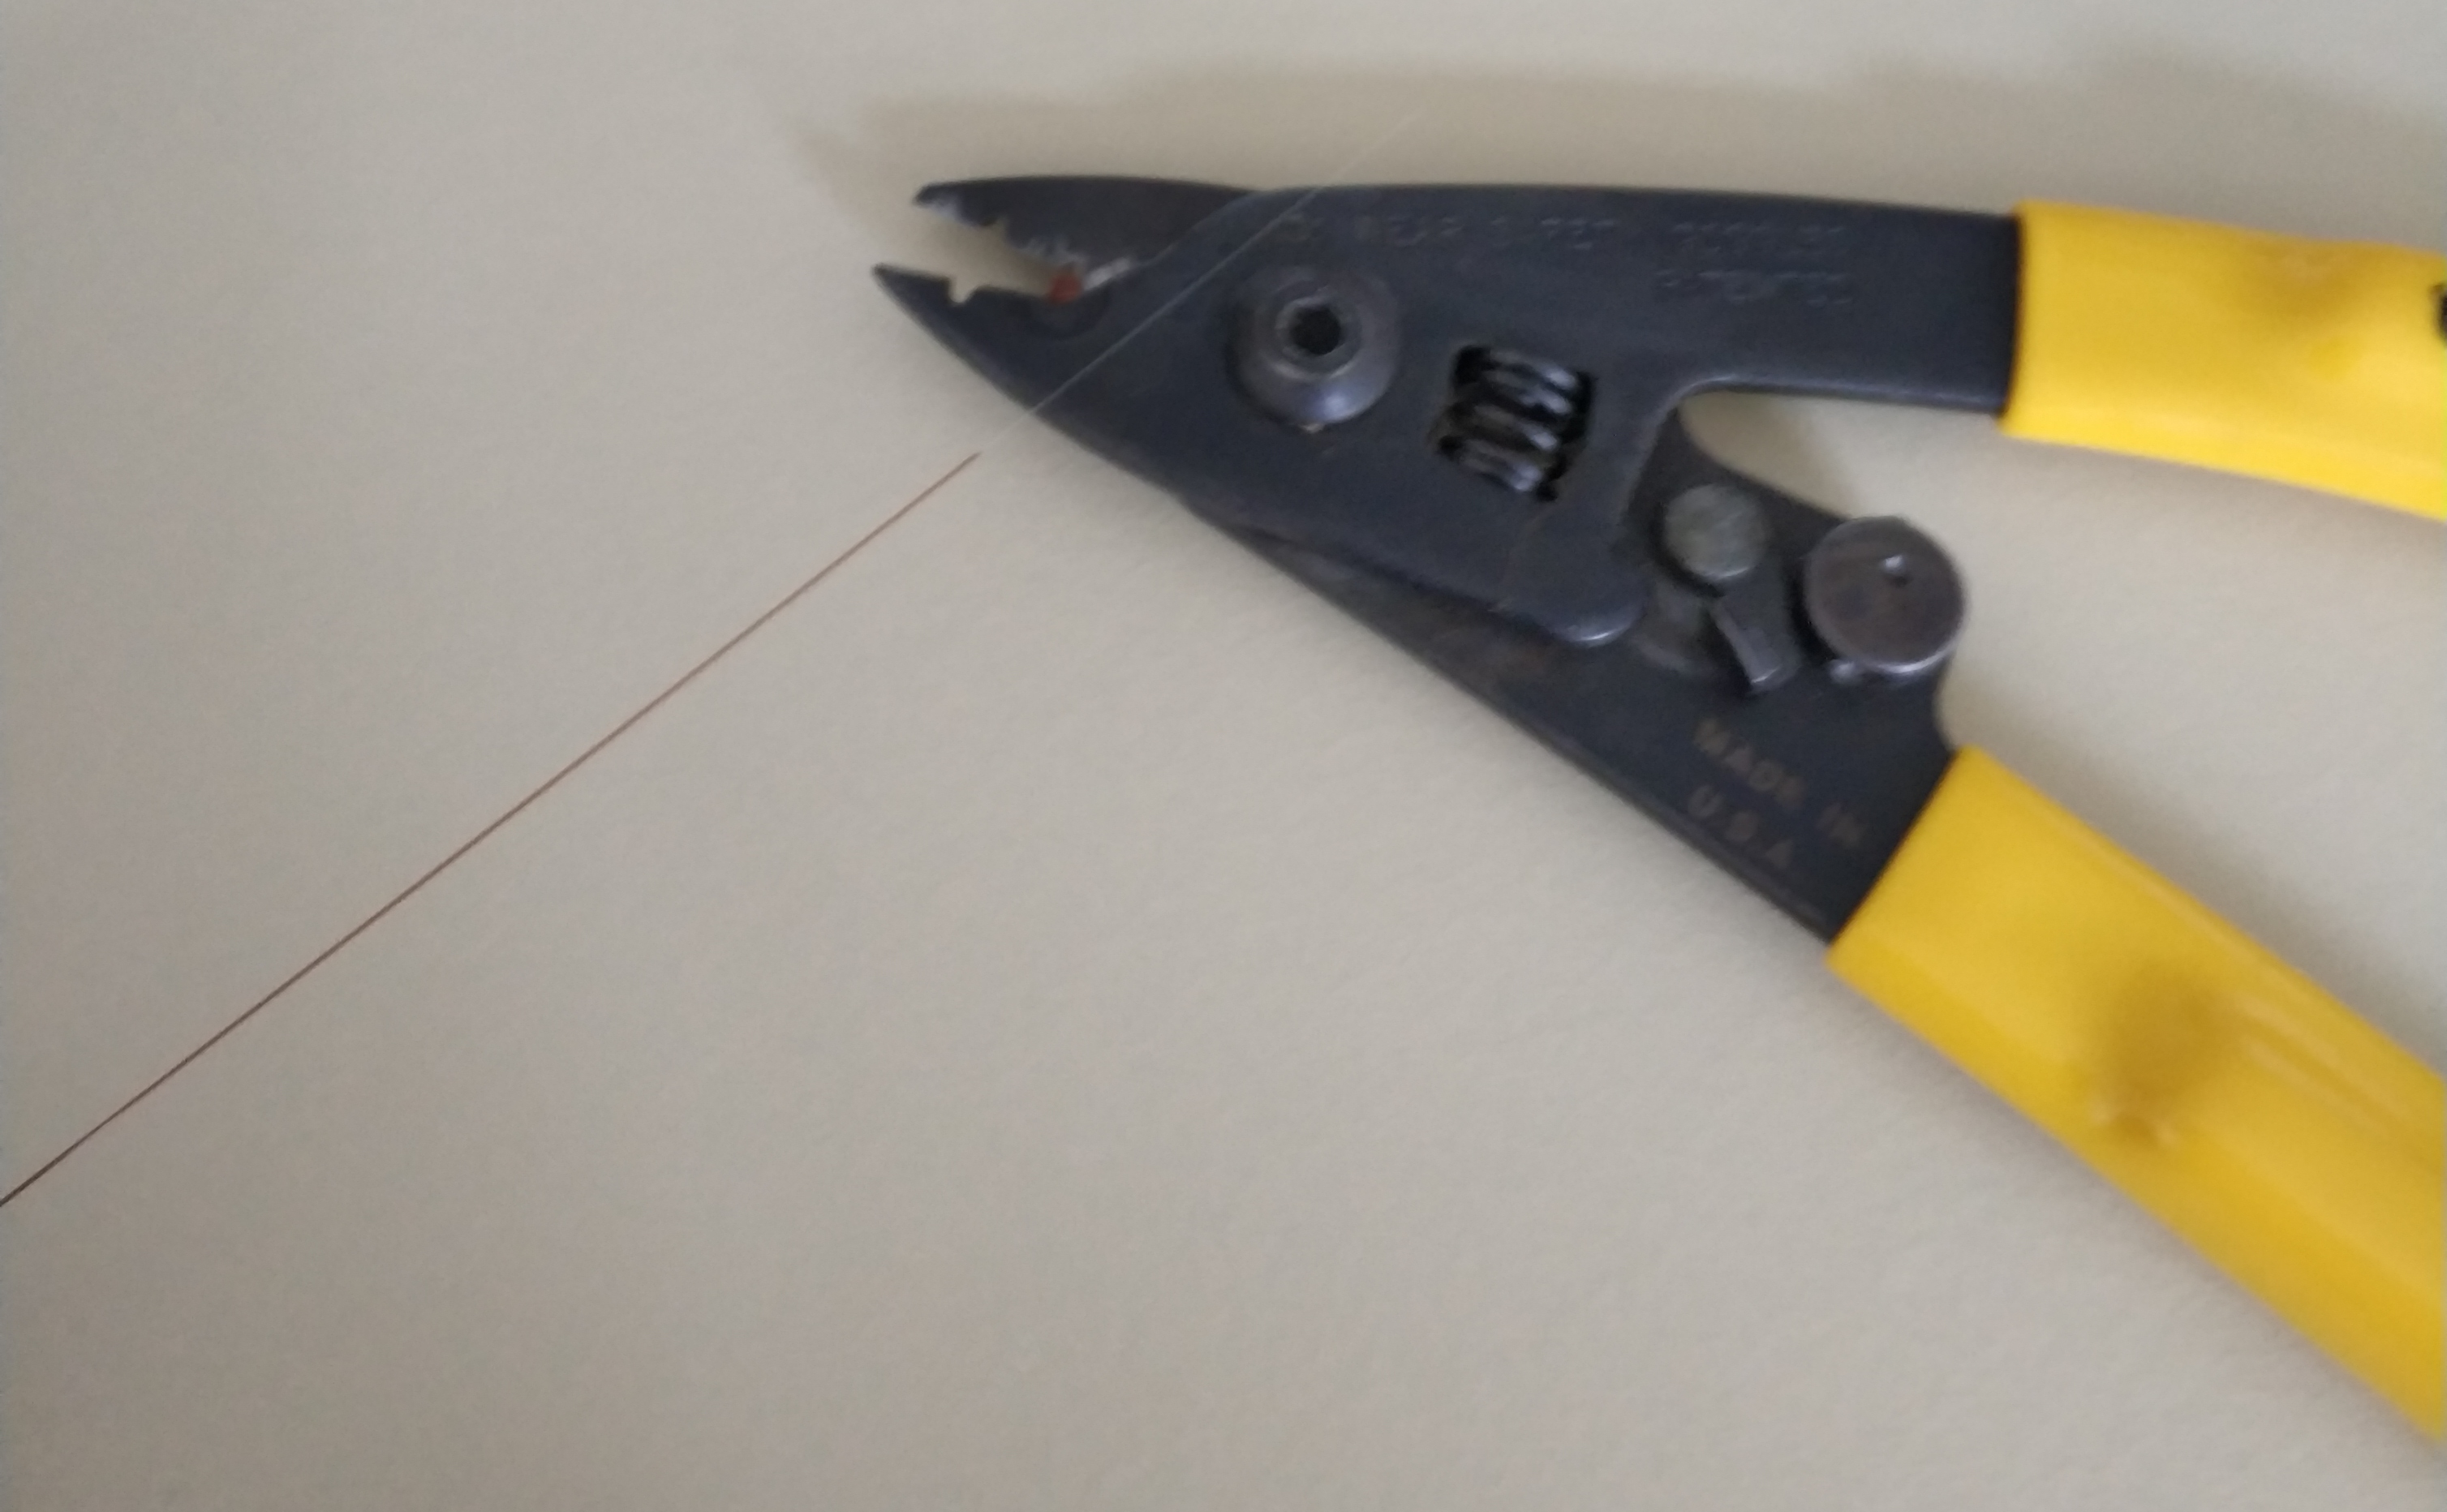
\includegraphics[width=0.618\textwidth]{graphics/milli.png}
%   \caption{Entfernen des Coatings mit Miller-Tool}
% \end{figure}

Mittels Cleaver konnten die Enden der Faser plan abgeschnitten werden. Dabei musste darauf geachtet werden, dass sie spannungsfrei in die Nut des Cleavers eingelegt, sowie, dass beim Öffnen des Cleavers und Herausnehmen der Faser diese festgehalten wurde.\\

\begin{figure}[H]
\centering
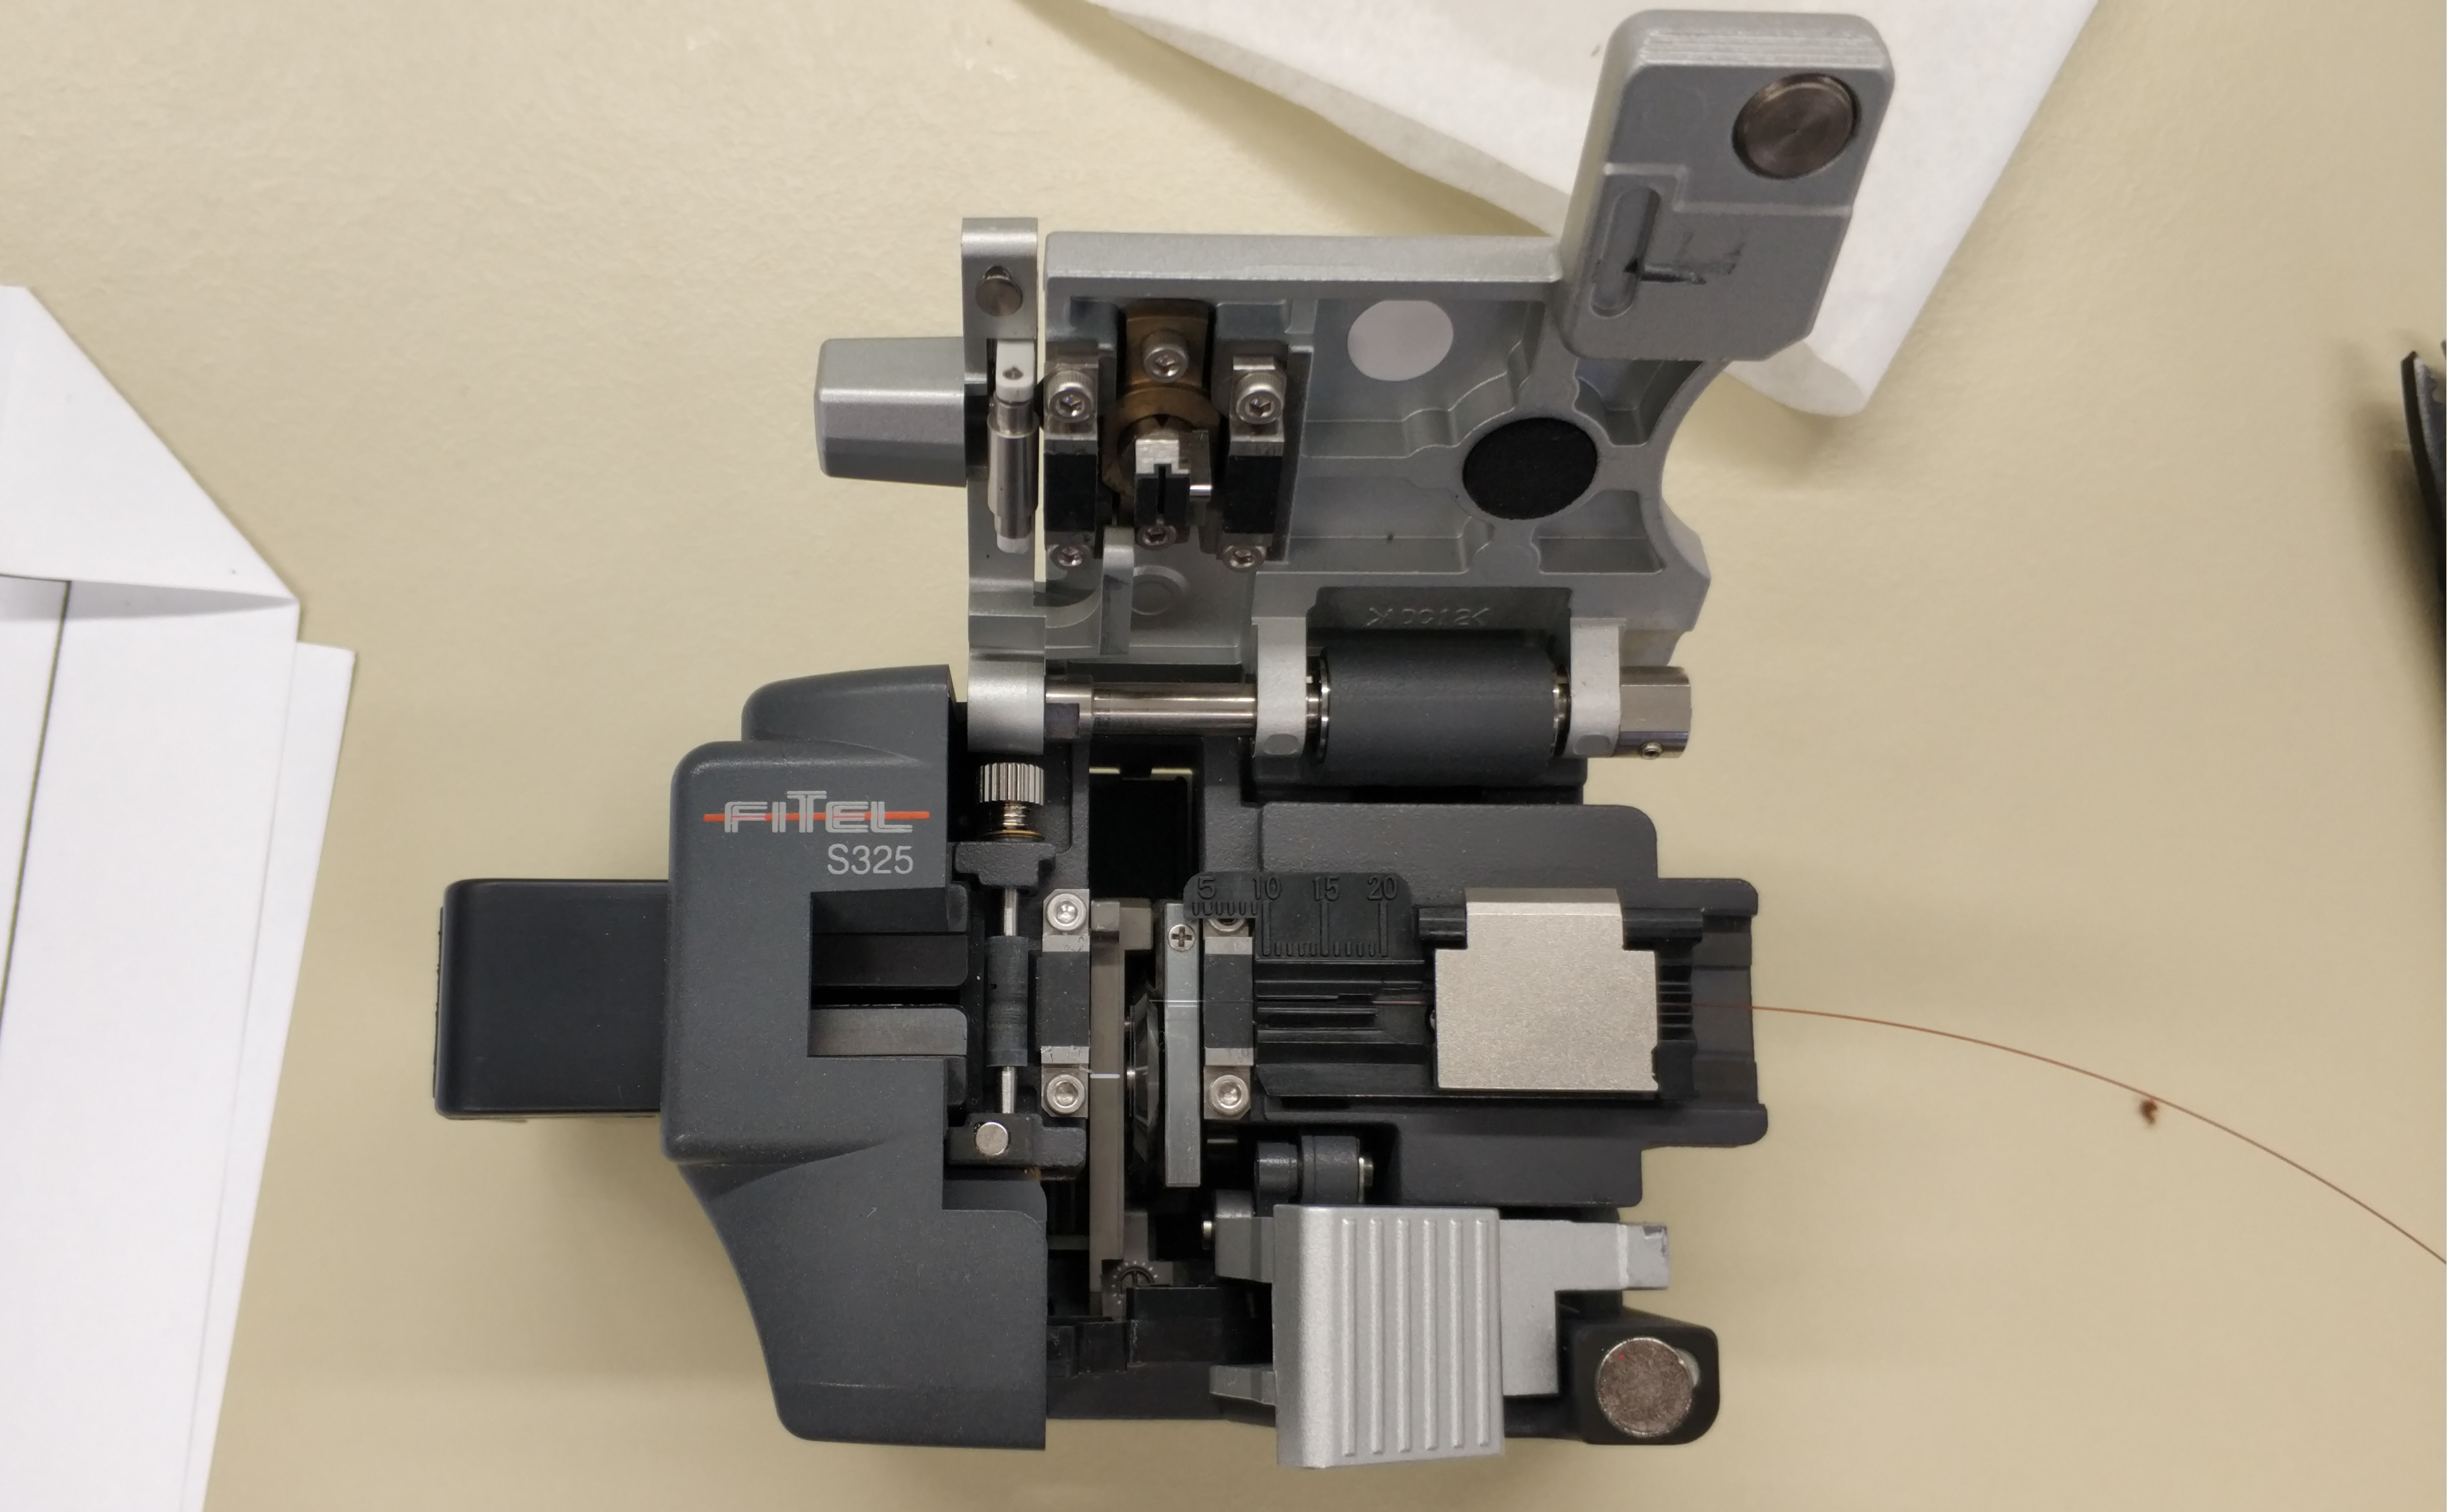
\includegraphics[width=0.618\textwidth]{graphics/cleavi.jpg}
\caption{Der Cleaver dient als Trennvorrichtung für die Faser}
\end{figure}


Nach dem Abschneiden durfte die Faser in keinen Kontakt zu anderen Oberflächen kommen, um erneute Verschmutzungen zu vermeiden.\\

Nun konnten die Enden in das Lichtbogenspleißgerät in die Nähe der Spleißelektroden gelegt werden. Dies erfolgte ähnlich wie beim Cleaver. Mit dem Schließen des Deckels wurde auf dem Display eine Mikroskopaufnahme beider Fasern angezeigt.\\

Voreinstellungen am Gerät bezüglich Durchmesser etc. wurden durch den Praktikumsbetreuer vorgenommen. Die automatische Ausrichtung der Faserenden zueinander wurde zu Übungszwecken abgeschaltet. Nach Einstellen der Schrittweite konnten die Fasern manuell in x-, y- und z-Richtung mit Referenz zum Mikroskopbild positioniert werden. Auf den vorläufigen Lichtbogen zur Beseitung von Verunreinigungen folgte das tatsächliche Spleißen der Faserenden. Das Ergebnis wurde mithilfe des Bildschirmes überprüft und ließ keine Mängel beanstanden.

\begin{figure}[H]
\centering
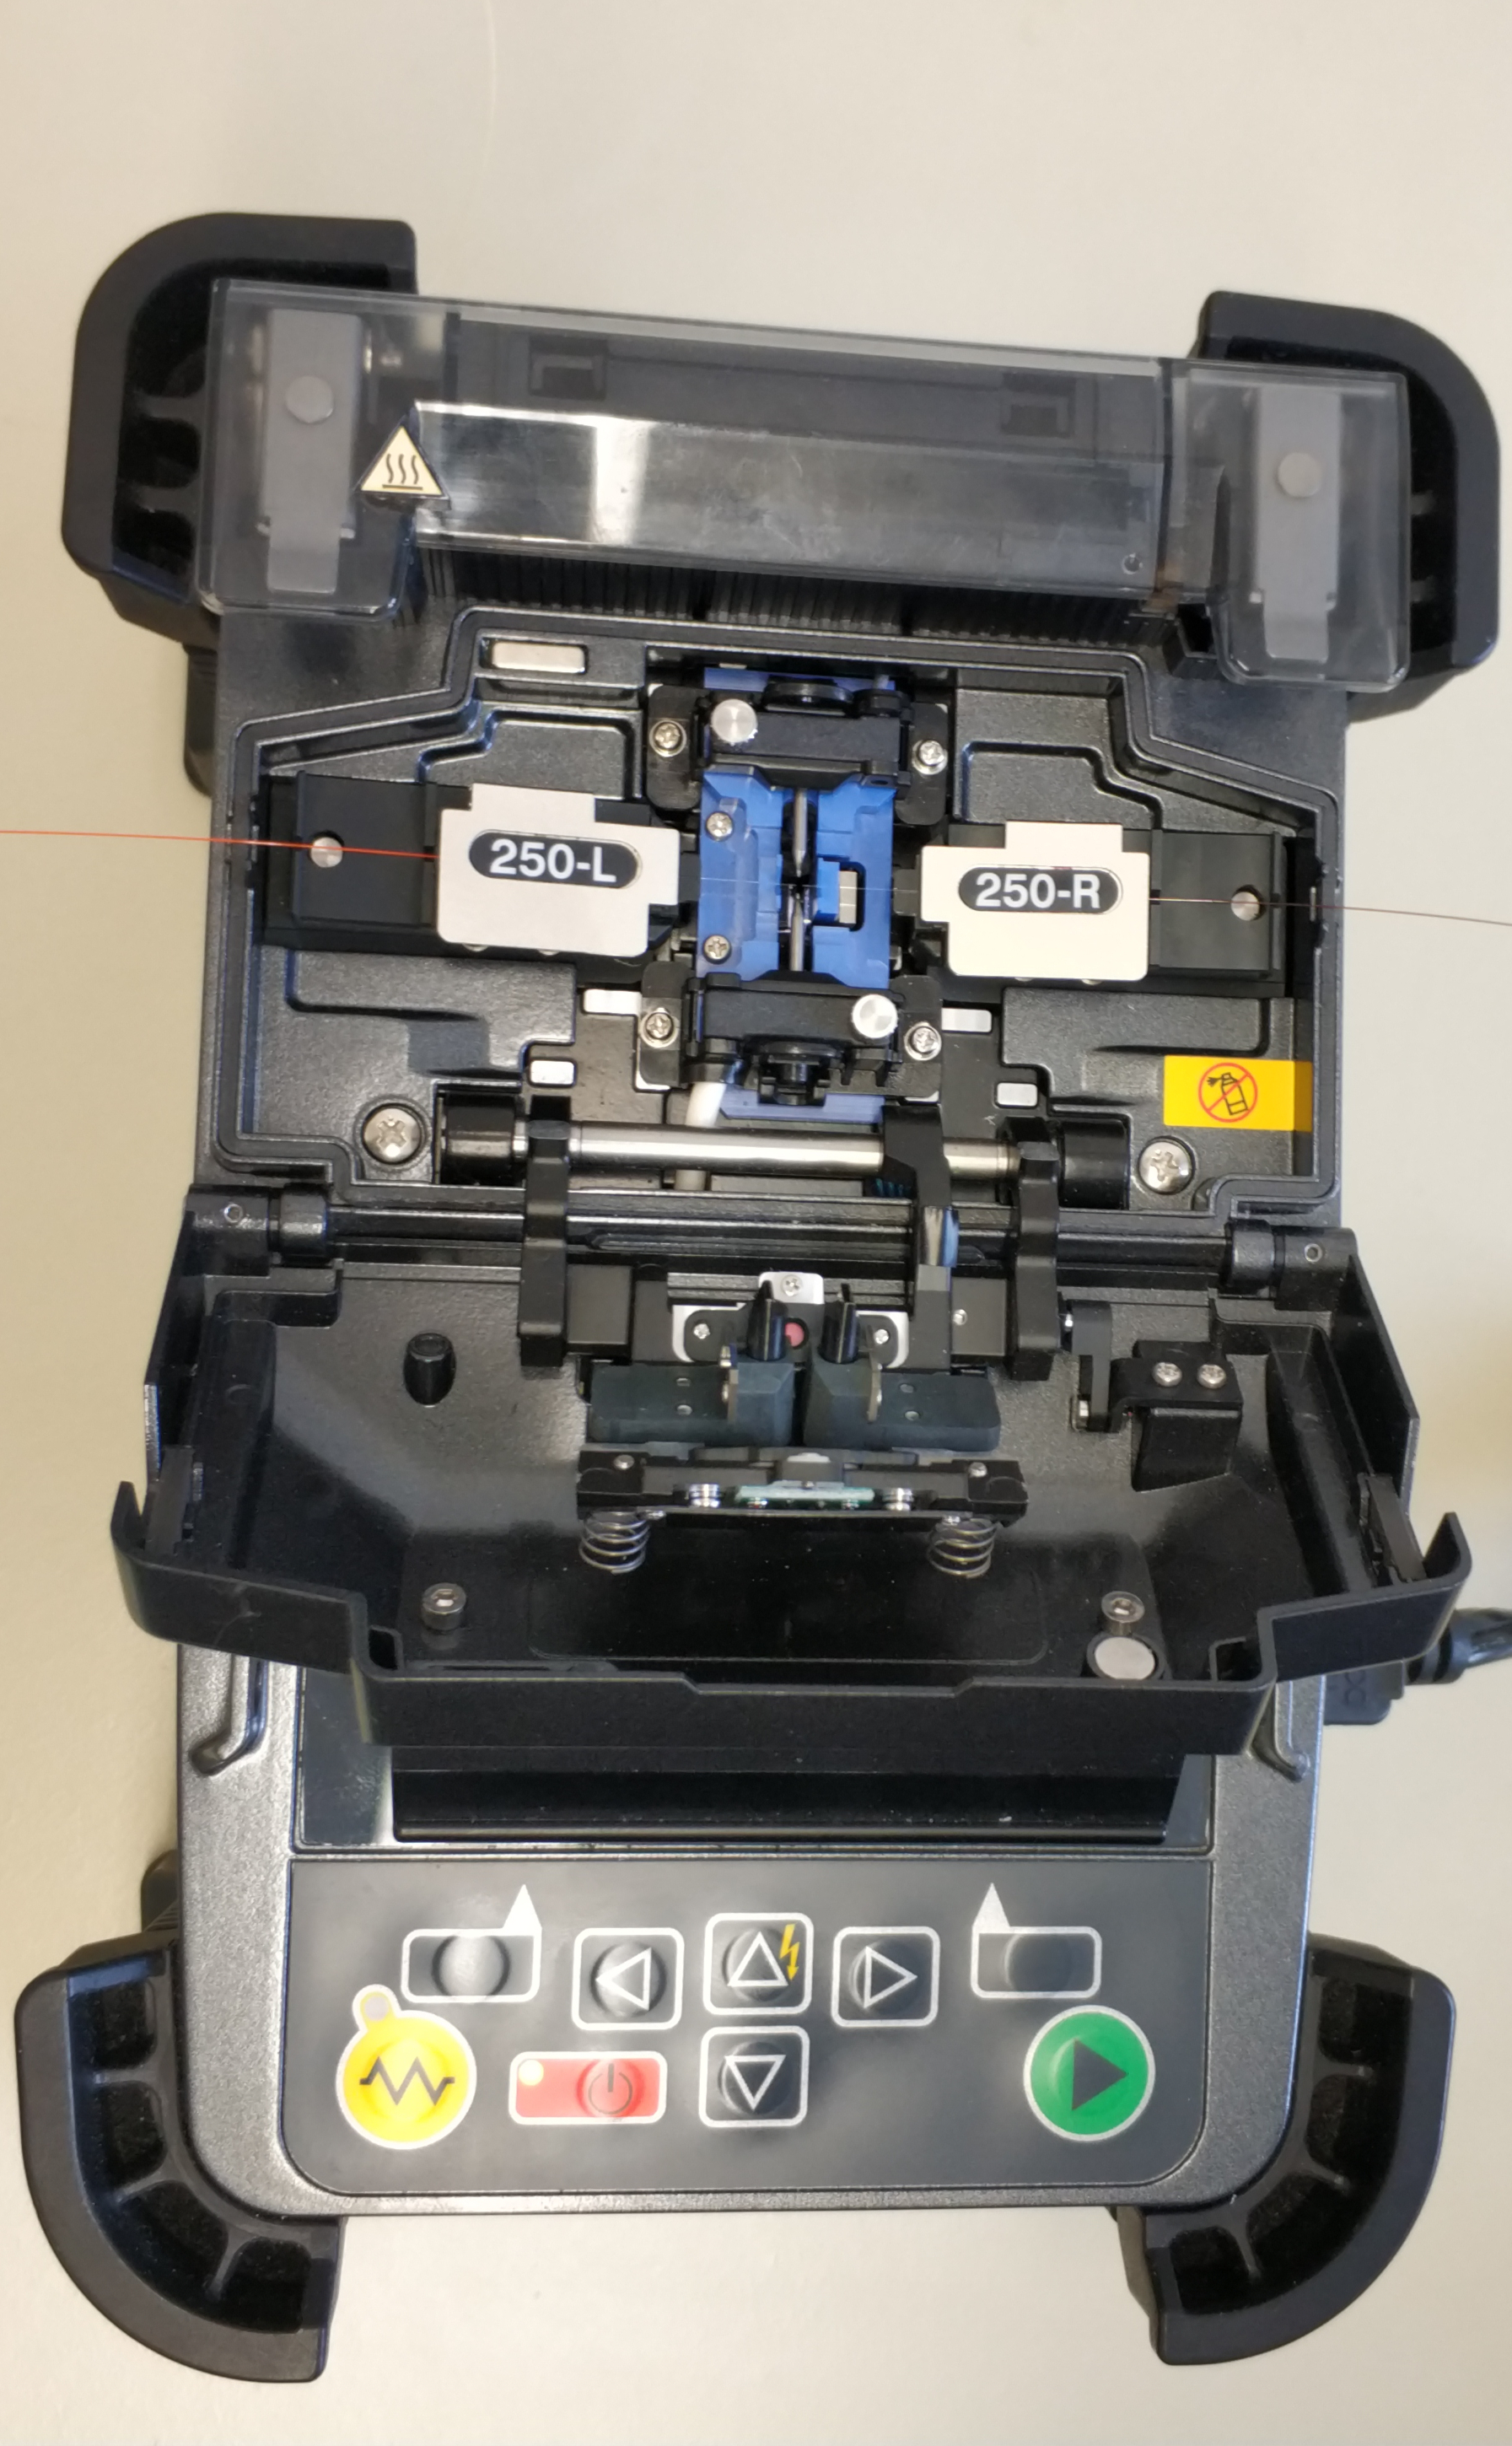
\includegraphics[width=0.382\textwidth]{graphics/spleisen.jpg}
\caption{Das Lichtbogenspleißgerät mit beiden Fasern}
\end{figure}

\begin{figure}[H]
\centering
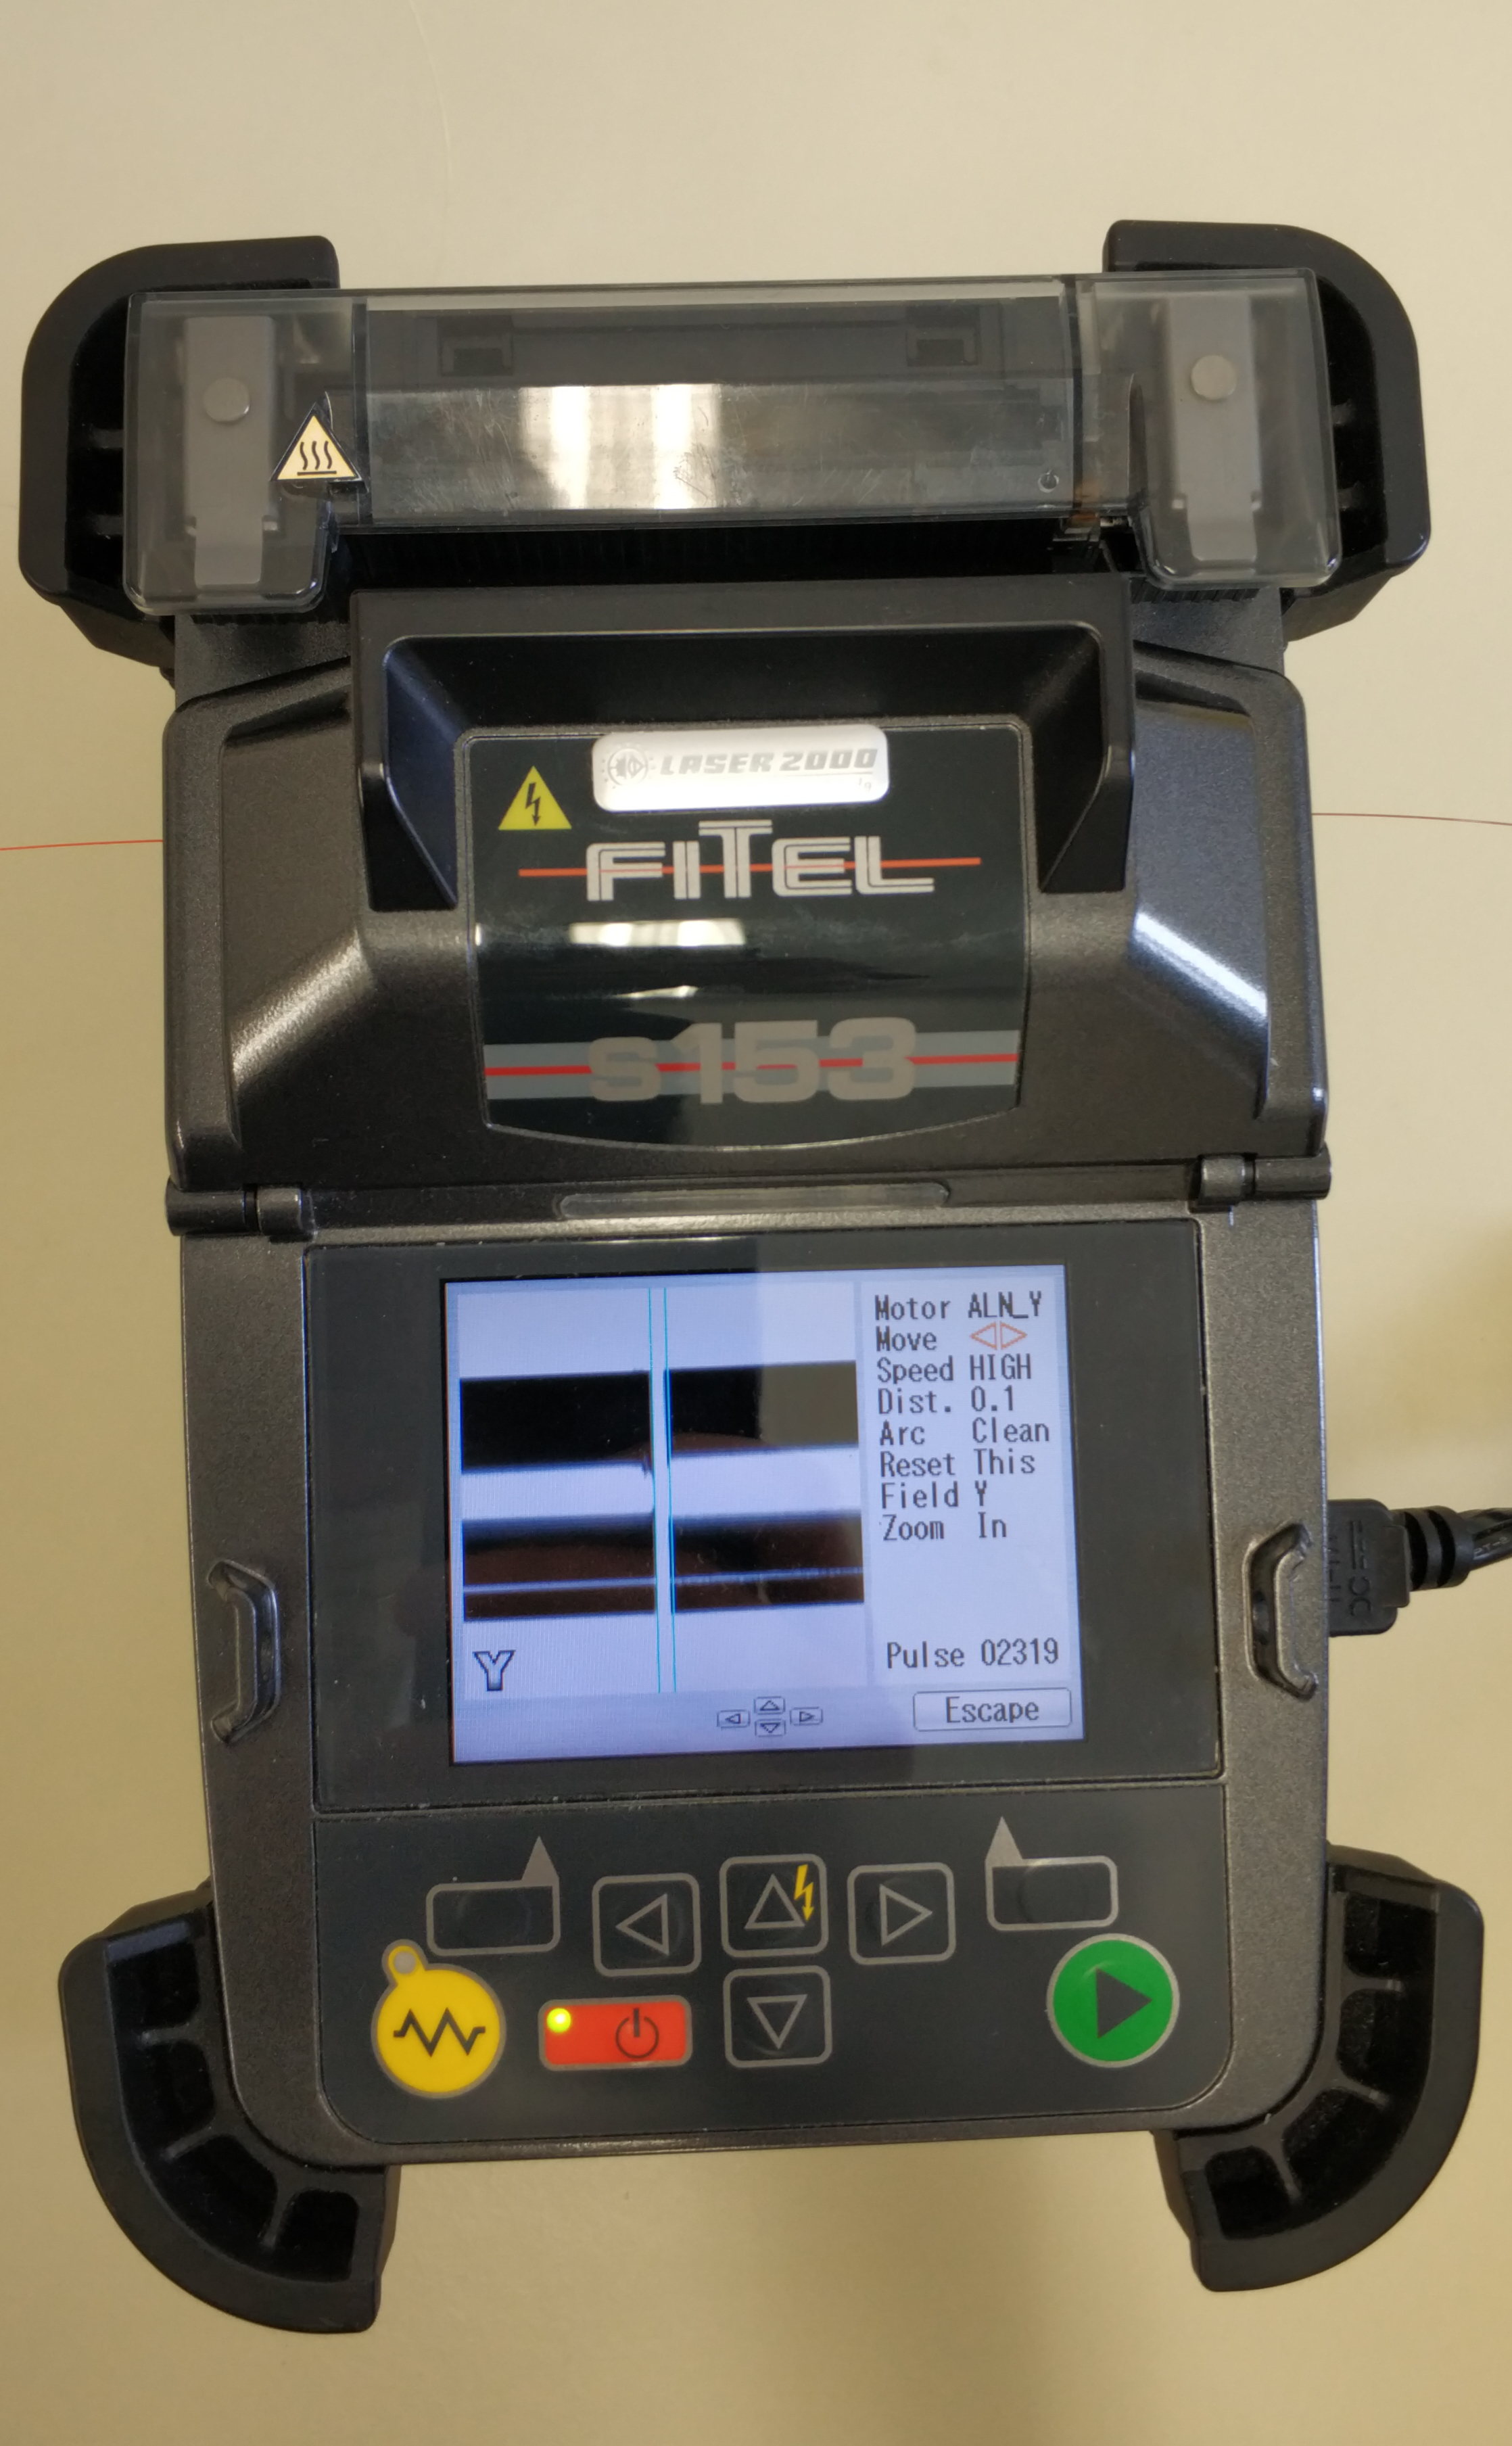
\includegraphics[width=0.382\textwidth]{graphics/spleisen2.jpg}
\caption{Anzeige des Mikroskopbildes und der Einstellungen auf dem Bildschirm des Spleißgerätes}
\end{figure}

Zur Verbesserung des Spleißergebnisses müssten extrinsische Faktoren analyisiert und minimiert werden (siehe Vorbereitungsaufgaben).

\subsection{Schutz der Spleißverbindung}
Der mechanische Schutz der Verbindung wurde im Praktikum nicht durchgeführt.

\subsection{Dämpfungsmessung an der vorgegebenen LWL-Strecke}
Für die Messung wurde eine auf zwei Trommeln aufgewickelte Faser verwendet. Mit einem Handpegelsender (optische Quelle) konnten zwei verschiedene Wellenlängen, 1310 $\si{\nano\meter}$ und 1550 $\si{\nano\meter}$, sowie die Modulationsart von CW (Continuous Wave) bis $2\,\si{\kilo\hertz}$ mit $50 \, \si{\percent}$ Duty Cycle bei einer Leistung von $-7 \, \si{\deci\bel}\text{m} \approx 200 \, \si{\micro\watt}$\  eingestellt werden.
Die Einfügedämpfung $D$ ist dann einfach die Differenz zwischen gesendeter und empfangener Leistung.
Die Ergebnisse sind in Tablle 2 sowie Tabelle 3 zu sehen.


\begin{table}[H]
  \centering
    \begin{tabular}{
    >{\columncolor{gray-0}}r rr}
                        & \cellcolor{gray-0}$P_{\text{Empfang}}$ & \cellcolor{gray-0}$D$ \\
    CW                    & $-8.64 \, \si{\deci\bel}\text{m}$            & $1.64\,\si{\deci\bel}$                       \\
    $270\,\si{\hertz}$    & $-11.66 \, \si{\deci\bel}\text{m}$           & $3.66\,\si{\deci\bel}$                       \\
    $1\,\si{\kilo\hertz}$ & $-11.66 \, \si{\deci\bel}\text{m}$           & $3.66\,\si{\deci\bel}$                       \\
    $2\,\si{\kilo\hertz}$ & $-11.66 \, \si{\deci\bel}\text{m}$           & $3.66\,\si{\deci\bel}$
    \end{tabular}
    \caption{Messwerte für $\lambda = 1310 \, \si{\nano\meter}$}
\end{table}

\begin{table}[H]
  \centering
\begin{tabular}{
>{\columncolor{gray-0}}r rr}
       & \cellcolor{gray-0}$P_{\text{Empfang}}$ & \cellcolor{gray-0}$D$ \\
CW     & $-8.54 , \si{\deci\bel}\text{m}$    & $1.54 , \si{\deci\bel}$   \\
270 Hz & $-11.58 , \si{\deci\bel}\text{m}$   & $4.58 , \si{\deci\bel}$   \\
1 kHz  & $-11.58 , \si{\deci\bel}\text{m}$   & $4.58 , \si{\deci\bel}$   \\
2 kHz  & $-11.58 , \si{\deci\bel}\text{m}$   & $4.58 , \si{\deci\bel}$
\end{tabular}
\caption{Messwerte für $\lambda = 1550 \, \si{\nano\meter}$}
\end{table}

Auffällig ist, dass die Dämpfung im Falle der modulierten Signale unabhängig von der Frequenz ist und sich vor allem um genau $-3 \, \si{\deci\bel}$ vom CW-Wert unterscheidet. Das ist darauf zurückzuführen, dass die Modulation mit einem Duty Cycle von $50 \si{\percent}$ erfolgt und daher in der selben Zeit auch nur $50\,\si{\percent}$ der Energie im Vergleich zum CW-Betrieb am Empfänger erscheint, wodurch die Leistung um die Hälfte oder $3 \, \si{\deci\bel}$ sinkt (Quelle $\rightarrow -10 \, \si{\deci\bel}\text{m}$).

Außerdem ist zu erkennen, dass die Dämpfung bei niedrigerer Wellenlänge höher ist und dabei frequenzunabhängig bleibt.
(Niedrigere Wellenlänge $\rightarrow$ höhere Dämpfung (Modendispersion größer))

\subsubsection{Active Alignment}
Der LWL wurde aufgetrennt und die Faserenden wurden für die Messung vorbereitet, in das Spleißgerät gelegt und aneinandergeführt jedoch ohne sie zusammenzuspleißen. Mit dem gleichen Messaufbau wie oben wurde die möglichst optimale Ausrichtung der Fasern über die Messung der maximalen Empfangsleistung $P_{\text{empf}_{\text{opt}}}$ bei $\lambda = 1310 \, \si{\nano\meter}, \text{CW}$ eingestellt. Bei einer Schrittweite von $0.1 \, \si{\micro\meter}$ wurde zuerst die x-Orientierung optimiert, es ergab sich

\[P_{\text{empf}_{\text{opt}_{x}}} = -11.2 \, \si{\deci\bel}\text{m}.\]

Nach Ausrichtung der y-Orientierung ergab sich der Endwert
\[P_{\text{empf}_{\text{opt}}} = -9.4 \, \si{\deci\bel}\text{m}.\]

\begin{figure}
\centering
\includegraphics[width=0.618\textwidth]{graphics/messi.jpg}
\caption{Messaufbau zur Dämpfungsmessung}
\end{figure}

\subsubsection{Leistungsprofil}
Nach dem vorher durchgeführten Active Alignment sollte nun die Leistung in Abhängigkeit von der Verschiebung vom Optimalpunkt (Zentrum) bestimmt werden. Mit einer Schrittweite von $1 \, \si{\micro\meter}$ ergaben sich die in Tabelle ?? aufgeführten Werte. Durch die Differenzbildung zur Leistung bei der Verschiebung $0$ kann ein relatives, leistungsunabhängiges Maß für den Dämpfungszuwachs in Abhängigkeit vom Abstand zum Zentrum ermittelt werden.

\begin{table}[H]
  \centering
\begin{tabular}{rrr}
\rowcolor{gray-0}
$\Delta r\ \text{in} \ \si{\micro\meter}$ & $P_{\text{Empfang}} \ \text{in} \ \si{\deci\bel}\text{m}$ & $ P_{\text{Empfang}} - P_{\text{opt}} \ \text{in} \ \si{\deci\bel}$ \\
\cellcolor{gray-0}0         & -9.42                                   & 0                                          \\
\cellcolor{gray-0}1         & -10.04                                  & -0.62                                      \\
\cellcolor{gray-0}2         & -11.09                                  & -1.67                                      \\
\cellcolor{gray-0}3         & -12.46                                  & -3.02                                      \\
\cellcolor{gray-0}4         & -14.1                                   & -4.68                                      \\
\cellcolor{gray-0}5         & -16.37                                  & -6.95                                      \\
\cellcolor{gray-0}6         & -19.25                                  & -9.83                                      \\
\cellcolor{gray-0}7         & -22.25                                  & -12.83                                     \\
\cellcolor{gray-0}8         & -25.8                                   & -16.38                                     \\
\cellcolor{gray-0}9         & -29.37                                  & -19,95                                     \\
\cellcolor{gray-0}10        & -32.78                                  & -23.36                                     \\
\cellcolor{gray-0}11        & -36.1                                   & -26.68                                     \\
                                  &                                         &
\end{tabular}
\end{table}

\begin{figure}
\centering
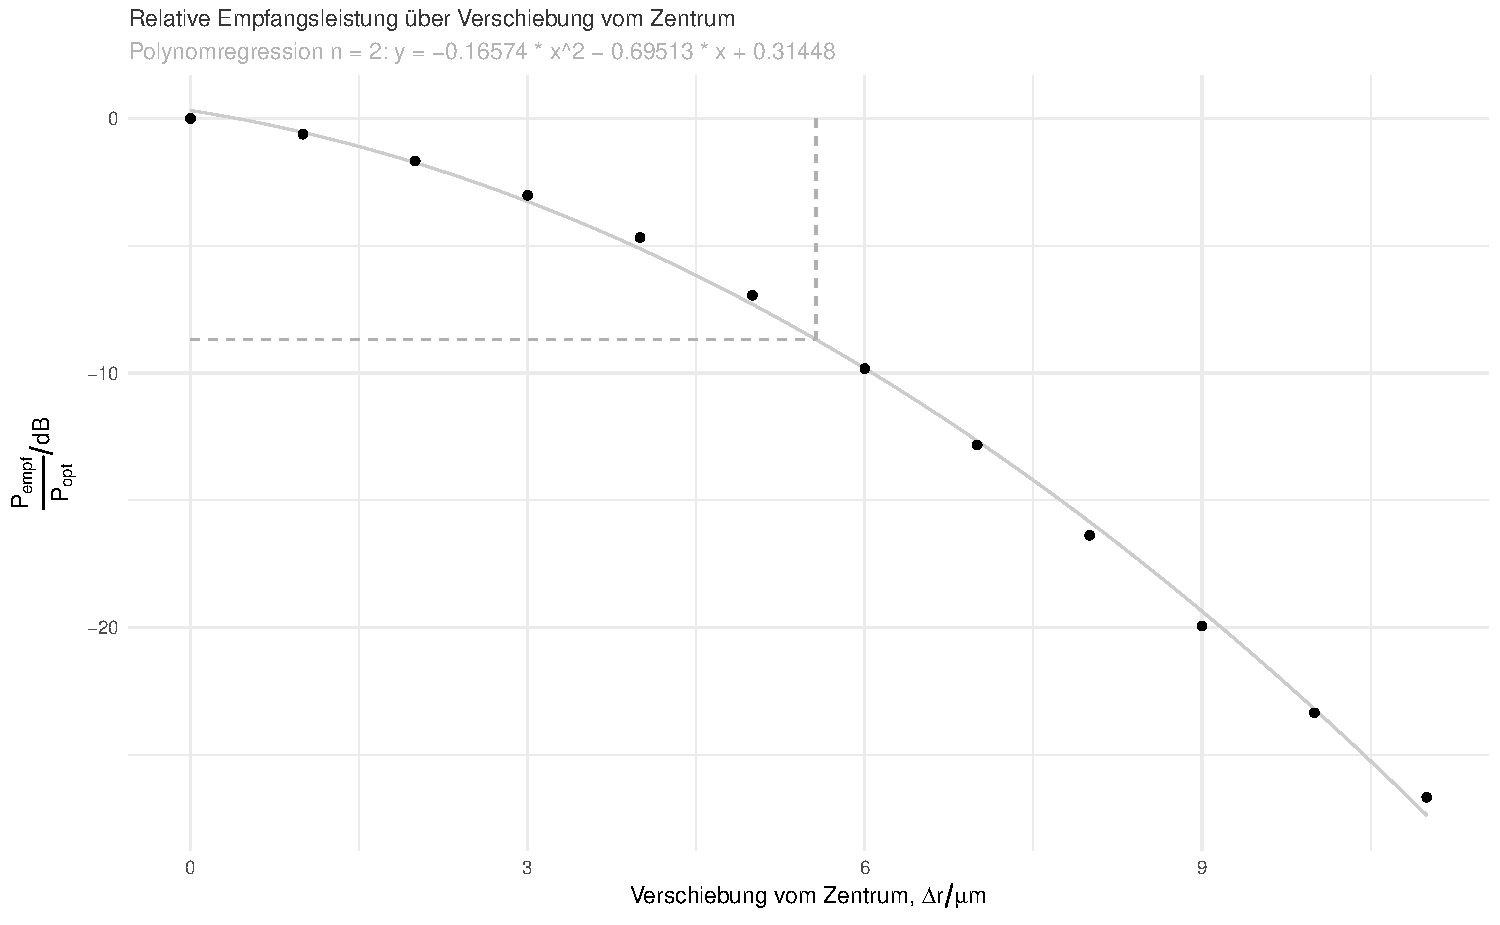
\includegraphics[width=\textwidth]{graphics/leistungsprofil/leistungsprofil.pdf}
\caption{Relative Empfangsleistung über Verschiebung vom Zentrum. Gestrichelte Linien kennzeichnen Modenfeldradius $\omega_{0}$}
\end{figure}

Mithilfe einer quadratischen Regressionsfunktion und deren Umkehrfunktion

\[x(y) = \frac{-b \pm \sqrt{b^{2} - 4a(c-y)}}{2a}\]

wurde die Verschiebung  ermittelt, bei der die Leistung zum Optimalpunkt um $\frac{1}{e^{2}} \approx 0.1354$ abgefallen ist, dies entspricht $-8.69 \, \si{\deci\bel}$. Dieser Abstand $\omega_{0}$ wird \emph{Modenfeldradius} genannt.

\[\text{MFR} \approx 5.565 \, \si{\micro\meter} \]

Da hier Singlemode-Fasern mit einem Durchmesser von $9 \, \si{\micro\meter}$ verwendet wurden, ergibt sich das Verhältnis von Modenfeldradius zu Faserradius zu

\[\frac{5.565 \, \si{\micro\meter}}{4.5 \, \si{\micro\meter}} = 1.24.\]


\subsection{Spleißmessung}
Die Faserenden wurden wie in der Aufgabenstellung auf den Optimalpunkt justiert und verspleißt. Nachfolgend wurde die Empfangsleistung gemessen.
\[P_{\text{empf}} = -9.13 \, \dBm\]
Da die Leistung der ungespleißten Faser mit $P_{\text{sender}} = -8.64 \, \dBm$ aus 2.3 bekannt ist, beträgt die Dämpfung, die durch den Spleiß verursacht wird

\[D_{\text{Spleiss}} = 9.13 \, \dBm - (8.64 \, \dBm) = 0.49 \, \si{\deci\bel}\]

Es handelt sich hierbei nicht um intrinsische, sondern extrinsische Verluste, die durch den Spleißprozess eingebracht wurden, wie Verunreinigungen oder einen nichtidealen Abschnittwinkel. Gängige Werte der Spleißeinfügedämpfung liegen im Bereich von $0.02 \, \si{\deci\bel} .. 0.1 \, \si{\deci\bel}$ (\href{https://blog.energiedienst.de/spleissen/}{Quelle}). Unser Spleiss sollte also in einer echten Anwendung erneut durchgeführt werden.

\subsection{Dämpfung durch Faserbiegung}
Durch einen Knoten im LWL sollte der Einfluss von Makrobiegungen in Abhängigkeit vom Durchmesser des Knotens/ der Biegung ermittelt werden. Durch Makrobiegungen fallen die Lichtstrahlen mit einem Winkel kleiner dem Winkel der Totalreflexion auf die Kern-Mantel-Grenze und werden in den Mantel gebrochen. Der so entstehende Energieverlust spiegelt sich in einer Dämpfungserhöhung wieder.\\

Tablle 4 zeigt die Messwerte der empfangenen Leistung sowie der Dämpfung bezogen auf den Anfangswert (vernachlässigbare Dämpfung bei hohem Radius).
Man sieht, dass bei vergleichsweise großen Radien die Biegung kaum einen Einfluss auf die Dämpfung hat, jedoch ab einem Wert von $6.5 \, \si{\milli\meter}$ schnell ansteigt.

\begin{table}[H]
  \centering
\begin{tabular}{
>{\columncolor{gray-0}}rrr}
Kreisradius in mm & \cellcolor{gray-0}Empfangsleistung in \si{\deci\bel}\text{m} & \cellcolor{gray-0}Dämpfung in dB \\
45                & -9.13                                                                                                                      & 0                                      \\
31                & -9.13                                                                                                                      & 0                                      \\
20.5              & -9.13                                                                                                                      & 0                                      \\
12.5              & -9.13                                                                                                                      & 0                                      \\
8.5               & -9.19                                                                                                                      & 0.06                                   \\
6.5               & -9.86                                                                                                                      & 0.73                                  \\
4                 & -22.26                                                                                                                     & 13.13                                 \\
3                 & -53.4                                                                                                                      & 44.27                                 \\
2                 & -62.7                                                                                                                      & 53.57
\end{tabular}
\caption{Messwerte der Aufgabe 5.5}
\end{table}
